% Diese Zeile bitte -nicht- aendern.
\documentclass[course=erap]{aspdoc}

%%%%%%%%%%%%%%%%%%%%%%%%%%%%%%%%%
%% TODO: Ersetzen Sie in den folgenden Zeilen die entsprechenden -Texte-
%% mit den richtigen Werten.
\newcommand{\theGroup}{125} % Beispiel: 42
\newcommand{\theNumber}{A220} % Beispiel: A123
\author{Markus-Ionut Vrancea \and Kevin Kafexhi \and Ota Takushima}
\date{Wintersemester 2023/24} % Beispiel: Wintersemester 2019/20
%%%%%%%%%%%%%%%%%%%%%%%%%%%%%%%%%
\usepackage{csquotes}
\usepackage{verbatim}
\graphicspath{images}

% Diese Zeile bitte -nicht- aendern.
\title{Gruppe \theGroup{} -- Abgabe zu Aufgabe \theNumber}

\begin{document}
\maketitle
\section{Einleitung}
\paragraph{}
Die digitale Bildverarbeitung behandelt grundlegende Methoden zur Bearbeitung und Aufbereitung von Bildern. 
Die Bildverarbeitungstechniken haben sich in den letzten zehn Jahren aufgrund zahlreicher Anwendungsbereiche, 
des wissenschaftlichen Interesses an diesem noch relativ jungen Forschungsgebiet und der zunehmenden Leistungsstärke 
des Computers etabliert und verbessert. Themen wie Bildentrauschung, Segmentierung und Bildrekonstruktion sind in Bereichen 
wie der Nanotechnologie, der Sensorik und der medizinischen Bildgebung nicht mehr wegzudenken. Die Fernerkundung der Erde 
und des Universums, die aus militärischen Gründen motiviert wurde und ihre Bilder und Erkenntnisse in der Meteorologie, 
der Ozeanographie und der Astronomie anwendet, ist ein weiterer wichtiger Einsatzbereich.
Es ist möglich, die Informationen der Bilder aus diesen verschiedenen Aufnahmequellen zu bearbeiten und zu ändern.++ 

\subsection{Bildentrauschung}
\paragraph{}
Eins der wichtigsten Verfahren in der Bildverarbeitung ist die Bildentrauschung. Was macht die Durchführung einer 
Bildentrauschung so wichtig? Unerwünschte Störungen können bei der Aufzeichnung und Übertragung von Bildern das Bild
verfälschen und Informationen löschen. Der Versuch, die Störungen im Bild zu entfernen, beinhaltet nun die Wiederherstellung 
der Bildinformationen an den gestörten Stellen, indem die Informationen aus den umliegenden Pixeln verwendet werden. 
Nicht nur die Rauschentfernung, sondern auch die Kantenerhaltung, Erkennung und Extraktion sind bei der Modellierung 
eines effizienten Entrauschungsalgorithmus von entscheidender Bedeutung. Dass Bildkanten wichtige Informationsquellen 
sind, erklärt die Bedeutung dieser eng miteinander verbundenen Aufgaben bei der Verzerrung des Bildes.

\clearpage


\begin{figure}[!h]
    \begin{center}
      \centering
      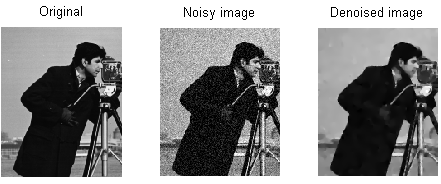
\includegraphics[scale=1.2]{images/ROF_Denoising_Example.png}
      \caption{ Ergebnis eines Bildes nach der Weichzeichnung und Entrauschung) \cite{Beispiel}}
    \end{center}
\end{figure}

\subsection{Aufgabenstellung}
\paragraph{}
Unsere Praktikumsaufgabe besteht darin eine effiziente Bearbeitungsweise zu finden, um ein farbiges Bild in Graustufen zu konvertieren 
und schließlich, mit Hilfe von dem Laplace-Filter und einer Weichbildung, das Bild zu entrauschen. Als Eingabe wird eine PPM Datei erwartet,
die dem Algorithmus übergeben wird. Nach dem Ausführen des Algorithmus wird das entrauschte Bild im PGM Format in einer separaten 
Ausgabedatei gespeichert. Unsere Lösung wird durch zwei verschiedene Implementierungen dargestellt. Die erste Implementierung ist 
die \verb|denoise| Funktion, welche die Bildentrauschung Schritt für Schritt für jeden Pixel ausführt.++ 
Unsere zweite Implementierung \verb|denoise_V1| stellt eine effiziente Methode dar, den Algorithmus durchzuführen, indem SIMD-Befehle 
benutzt werden. Zu diesem Zweck wird die Vorgehensweise des Algorithmus im theoretischen Teil analysiert und die Optimierung des 
Algorithmus im praktischen Teil beschrieben.


\section{Lösungsansatz}
++
\subsection{Theoretischer Teil}
\paragraph{}
Der folgende Abschnitt beschreibt den Ansatz unseres Programms, das eine PPM Datei erwartet und nach einer Sequenz von Verarbeitungen
 eine PGM Datei ausgibt.
Das PPM Bildformat (.ppm), das wir in diesem Projekt explizit als Eingabe behandeln werden, steht für \enquote{Portable Pixel Map} 
und ist ein Teil der Netpbm, ein Bildformat das in 1988  veröffentlicht wurde.++ Die Datei wird binär dargestellt und wird mit einem Header, 
das den Dateityp, die Breite, Höhe und die maximale Farbgröße des Bildes enthält, gefolgt von den Pixeln des Bildes, wo jede 3 Bytes einem 
Pixelwert entspricht. Das Format kann auf Grund ihrer Einfachheit innerhalb einer E-Mail Nachricht ohne besondere Kapselung übertragen werden,
sodass es möglichen Übersetzungen und Umkodierungen überleben kann und auf der anderen Seite leicht extrahierbar sein kann. cite 
Da dieses Format die Bilddatei Pixel für Pixel speichert und Gruppen von Pixeln derselben Farben nicht zusammenfasst, kann dies, 
im Vergleich zu modernen Formaten wie JPEG oder PNG, eine relative große Datei sein. 

Ein einfaches Beispiel des PPM Formats sieht wie folgt aus: \newline

\begin{center}
    \begin{verbatim}
    P6  
    # example from the man page
    4 4
    255
    0  0  0    0  0  0    0  0  0   15  0 15
    0  0  0    0 15  7    0  0  0    0  0  0
    0  0  0    0  0  0    0 15  7    0  0  0
    15 0 15    0  0  0    0  0  0    0  0  0
    \end{verbatim}
\end{center} cite

\begin{itemize}
    \item P6: Eine \enquote{magische Zahl} zur Identifizierung des Dateityps. Die magische Zahl eines PPM-Bildes sind die beiden 
    Zeichen \enquote{P6}.
    \item \#: Alle Zeichen von einem \enquote{\#} bis zum nächsten Zeilenumbruch sind ein Kommentar und werden ignoriert.
    \item 4 4: Die Breite und Höhe des Bildes in ASCII-Dezimalzahl, getrennt von einem Leerzeichen.
    \item 255: Der maximale Farbwert, wiederum in ASCII-Dezimalzahl. Für das Projekt ist er auf 255 festgelegt.
    \item Die unteren Nummern sind ein Raster von Zeilen in der Reihenfolge von oben nach unten. Jede Zeile besteht aus \{Breite\} 
    pixeln in der Reihenfolge von links nach rechts. Jedes Pixel ist ein Tripel von roten, grünen und blauen Mustern, in dieser Reihenfolge. Jedes Muster wird in reinem Binärformat durch 1 Byte dargestellt.
\end{itemize}

Eine 24bpp PPM Datei kann $2^{24} = 16777216$ Farben in RGB darstellen und jede Pixel lässt sich wie folgt darstellen:
\begin{center}
    \( p(x, y) = \begin{bmatrix} R \\ G \\ B \end{bmatrix} \)
\end{center}

++ Intro smoother
Das PGM Bildformat (.pgm) steht für \enquote{Portable GrayMap} und ist auch ein Teil der Netpbm. Dieses Format wird ebenfalls binär 
dargestellt und behandelt die Schwarz-Weiße Version der obengenannten PPM. Das Format  nutzt für ein Pixelwert nur 1 Byte. 
EXplain 
Da die Ausgabe unseres Programms in Graustufen erfolgt, haben wir uns entschieden, das PGM-Format als Ausgabe zu verwenden. 
(explain file smaller)
Das PGM Format ist ähnlich aufgebaut wie das PPM Format. Der Unterschied liegt an der Repräsentierung der Pixeln, 
die jetzt pro Pixel durch ein Byte dargestellt wird, statt 3 Bytes wie in einer PPM Datei. und die magische Zahl (explain better). 
Die Zeichen \enquote{P5} entsprechen dem PGM Format.

\subsubsection*{Graustufenkonvertierung}

\paragraph{}
Um die Graustufenkonvertierung durchzuführen wenden wir die folgende Formel für jeden Pixel an:

\begin{center}
    \( D = \frac{a \cdot R + b \cdot G + c \cdot B}{a + b + c} \)
\end{center}

wobei a, b und c Konstanten sind mit Werte:

\begin{center}
    \(a = 2.99, b = 5.87, c = 1.14\)
\end{center}

In dieser Formel wird die Gewichtung der rot, grün und blau Werte nach dem ITU-R BT.601 Standard Construction of Luminance eingestellt. 
Dieser Standard wurde von der International Telecommunication Union für die digitale Videocodierung definiert und dient als eine effiziente 
Gewichtung für die Graustufenfilterung. Der berechnete Durchschnitt wird dann Pixel für Pixel in die neue PGM Datei eingefügt.

\subsubsection*{Laplace Filter}

\paragraph{}
Das Graustufenbild wird dann einer Rauschreduzierung unterzogen, wofür wir zunächst den Laplace-Filter auf das Graustufenbild Q anwenden, 
der zur Kantendetektion verwendet wird. Wir definieren Kanten als eine große Farbänderung zwischen benachbarten Pixeln. 
Er operiert durch Anwendung einer bestimmten Faltungsmatrix mit der Dimension 3 auf jedem Pixel des Bildes und rechnet sich wie folgt:

\begin{center}
    \(Q^L \approx M^L * Q\)
        mit
    \(M^L = \begin{pmatrix} 
                0 & 1 & 0 \\
                1 & -4 & 1 \\
                0 & 1 & 0 \\
            \end{pmatrix}\)
\end{center}

\paragraph{}
Diese Faltungsmatrix hat eine hohe, negative zentrale Pixelgewichtung und kleinere Gewichtungen für die umgebenden Pixel. 
Dadurch werden Unterschiede in der Pixelintensität betont, was zur Verstärkung von Kanten führt. Wichtig zu beachten ist, 
dass bei den Kanten des Bildes für Zugriff außerhalb des Definitionsbereichs der Funktion implizit den Wert 0 angenommen 
wird und deswegen die Kanten nach der Anwendung des Filters dünkler werden.

\subsubsection*{Weichzeichnung}

\paragraph{}
Als nächsten Schritt berechnen wir mittels der folgenden Faltungsmatrix die Weichzeichnung des Bildes, in dem wir den 
Weichzeichnungsfilter auf das Graufstufenbild anwenden:

\begin{center}
    \(Q^W = \frac{1}{16} \cdot M^W * Q\) 
        mit 
    \(M^W = \begin{pmatrix} 
                1 & 2 & 1 \\
                2 & 4 & 2 \\
                1 & 2 & 1 \\
            \end{pmatrix}\)
\end{center}

\paragraph{}
Mit Ausnahme der Pixel an den Rändern oder Ecken des Bildes nimmt jedes Pixel das Produkt von den äußeren Pixelwerten 
und 1 oder 2, je nachdem, wo das Pixel um das mittlere Pixel herum platziert wird. Dazu wird noch das Produkt von dem 
mittleren Pixelwert und 4 addiert und zurückgegeben. Hier wird das mittlere Pixel von den umgebenden Pixeln beeinflusst, 
wodurch das Pixel unscharf wird. Diese Methode wird auch an Kanten verwendet, mit der Ausnahme, dass Matrixmultiplikationen 
für Pixel an Kanten nicht vergütet werden, da sie nicht vorhanden sind. Die Summe der an den Ecken werden durch 9, 
an den Kanten durch 12 und alle anderen Pixeln durch 16 geteilt. Diese Zahlen ergeben sich aus der Differenz 
von 16 und der Summe der Zahlen in der Matrix, die mit den fehlenden Positionen in der rechten Matrix multipliziert werden sollten.

\subsubsection*{Berechnung des entrauschten  Bildes}

\paragraph{}
Das entrauschte Bild ergibt sich dann indem man das originale und das weichgezeich-nete Bild basierend auf der Ausgabe des 
Laplace-Filters wie folgt kombiniert:

\begin{center}
    \(Q'_{(x, y)} = \frac{|Q_{(x, y)}^L|}{1020} \cdot Q_{(x, y)} + (1 - \frac{|Q_{(x, y)}^L|}{1020}) \cdot Q_{(x, y)}^W\)
\end{center}
\begin{center}
    \(\frac{|Q_{(x, y)}^L|}{1020} \cdot Q_{(x, y)}\) (1)
\end{center}
\begin{center}
     \((1 - \frac{|Q_{(x, y)}^L|}{1020}) \cdot Q_{(x, y)}^W\) (2)
\end{center}

(1): Diese Division normalisiert das Ergebnis des Laplace-Filters. Der Filter erzeugt Werte, die die Intensität der Kanten 
im Bild repräsentieren. Durch die Division wird dieser Wert in einen Faktor zwischen 0 und 1 umgewandelt und mit dem Graugestuften 
Bild multipliziert, was an Stellen, an denen das Laplace-gefilterte Bild hohe Werte hat,  die ursprünglichen Werte des Bildes behält, 
was auf scharfe Kanten hindeutet.

(2): Diese Operation bestimmt, wie viel vom weichgezeichneten Bild genutzt wird. An Stellen mit weniger Details oder Kanten wird 
mehr vom weichgezeichneten Bild genommen, was hilft, das Rauschen zu reduzieren.
Durch die Addition der beiden Seiten wird ein Bild ausgegeben, das bei den Kanten eines Bildes die Pixelwerte des originalen 
Bildes nimmt und sonst die weichgezeichneten Werten. Dies führt zu einem entrauschten Bild, bei dem die scharfen Kanten erhalten bleiben.

\subsection{Praktischer Teil}
\paragraph{}
In diesem Teil wird die Vorgehensweise der Implementierung einer Bildentrauschung beschrieben. Dafür werden zwei verschieden implementierte 
Funktionen verwendet. Die Hauptimplementierung beschreibt einen effizienten Algorithmus für die Bildentrauschung, während die 
Referenzimplementierung die normale Durchführung des Algorithmus darstellt. Dabei wird auch das Rahmenprogramm beschrieben, 
durch welches der Nutzer das Programm mit verschiedenen Optionen starten kann.

\subsubsection*{Rahmenprogramm}
\paragraph{}
Die Codebase besteht aus drei Quelldateien (\verb|.c|) und zwei  Headerdatei (\verb|.h|). Im Header (\verb|FileIO.h|) wird die Datenstruktur 
definiert, in welcher die Eingabedateien gespeichert werden. Die Eingabedatei ist durch ein struct representiert, welcher die Dimensionen 
des Bilds, wie auch den maximalen Farbwert, gefolgt von einem Pointer, der auf die Werte jedes Pixels zeigt, speichert. Die Definition der
Funktionen, die für die eigentliche Bildrauschung benutzt werden, kann man in der \textit{ImageDenoiser.h} Datei finden, während die einzelnen
Implementierungen in der \textit{ImageDenoiser.c} Datei gefunden werden können. In der \verb|main.c| Datei ist die Main-Methode vorhanden,
die das eigentliche Programm ausführt.
Die Command Line ermöglicht es dem Nutzer das Programm mit mehreren Parametern auszuführen. Dabei sind die Ein-/Ausgabe Parameter
(\verb|-i|, \verb|-o|), gefolgt von den entsprechenden Dateien immer anzugeben. Als Alternative kann sich der Nutzer mit dem Kommando 
\enquote{-h} oder \enquote{--help} auch eine Anweisung zur Nutzung der Parameter in der Konsole anzeigen lassen. Um die ausgeführte 
Version der Implementierung auszuwählen, muss der Parameter \verb|-V| gefolgt von einer 0 (\textit{Hauptimplementierung}) oder 1 
(\textit{Referenzimplementierung}) angegeben werden. Falls dieser Parameter nicht angegeben wird, wird per default die Hauptimplementierung
ausgeführt. Die Koeffizienten für die Graustufenkonvertierung können durch den \verb|--coeffs| Parameter angegeben werden. Falls dieser
Parameter nicht vom Nutzer angegeben wird, werden die default Werte a = 2.99, b = 5.87 und c = 1.14 verwendet. Um die Performanz der
Methode zu testen, muss zusätzlich der \verb|-B| Parameter angegeben werden. Nach dem Ausführen des Programms wird in diesem Fall die 
Laufzeit der Funktion in Sekunden in der Konsole angezeigt werden. Falls man die gesamte Laufzeit für mehrere Iterationen berechnen möchte,
muss man dem \verb|-B| Parameter zusätzlich noch eine positive Zahl, grösser als 0, hinzufügen. Diese Zahl gibt die Anzahl der durchzuführenden
Iterationen an. Zusätzlich wurde der Parameter \verb|-k| implementiert, der die Ausgabedateien beider Methoden vergleicht, um die Korrektheit
der Methoden zu testen.

\subsubsection*{Implementierung}
\paragraph{}
Als eine Programmiersprache ist C relativ hardwarenah und eignet sich daher hervorragend zum Schreiben effizienter Programme. 
Insbesondere nutzen wir für unser Bildenträuschungsprogramm Single Instruction, Multiple Data (SIMD), um mehrere Pixelwerte 
gleichzeitig zu verarbeiten. Diese Methode ist besonders vorteilhaft für Matrixoperationen, die einen Großteil unserer 
Entrauschungslogik ausmachen. Da für jede Matrixmultiplikation das Ergebnis der Berechnungen der Pixeln unabhängig voneinander sind, 
kann dies effektiv parallelisiert werden.
Unser Programm beinhaltet zwei Versionen: \verb|denoise()| und \verb|denoise_V1()|. Während \verb|denoise()| eine sequenzielle 
Bearbeitung der Pixel für alle Methoden durchführt, nutzt \verb|denoise_V1()| SIMD-Operationen für fast alle Schritte außer der
letzten Berechnung. Die Graustufenkonvertierung in \verb|denoise_V1()| verarbeitet vier Pixel gleichzeitig, und die Matrixmultiplikationen 
für die Laplace-Filter und die Weichzeichnung werden mit acht Pixeln gleichzeitig durchgeführt. Bei der Bearbeitung von Kanten und Ecken,
den sogenannten Edge Cases, greift das Programm jedoch auf die Pixel-für-Pixel-Bearbeitung zurück.



% TODO: Je nach Aufgabenstellung einen der Begriffe wählen
\section{Korrektheit/Genauigkeit}
\paragraph{}
Die Korrektheit unseres Programms wird durch eine Äquivalenzprüfung nachgewiesen. In unserem Programm wird dies durch zwei verschiedene 
Ansätze für dasselbe Problem erreicht. Der erste Ansatz ist in der Methode \verb|denoise| enthalten, die aus dem Ausgangsbild ein Graubild
berechnet, darauf einen Laplace-Filter anwendet, eine Unschärfe für das Graubild berechnet und dann alle drei Ergebnisse kombiniert. 
Dieser Ansatz folgt der mathematischen Lösung aus der Übung, die die Schritte wie zuvor beschrieben berechnet. Die andere Lösung ist
ein völlig anderer Ansatz für dasselbe Problem. Anstatt eine einfache Berechnung zu verwenden, haben wir SIMD verwendet und eine
weitere Methode namens \verb|denoise_V1| erstellt. Im Rahmenprogram gibt es eine Option -k, die der Benutzer verwenden kann. 
Falls diese Option gesetyt ist, werden beide Methoden \verb|denoise| und \verb|denoise_V1| aufgerufen, die Ausgabewerte beider
Methoden in verschiedenen Variablen a (für denoise) und b (für denoiseV1) gespeichert und die beiden Ausgabedateien Byte für 
Byte vergliechen. Wir haben die Ergebnisse für eine Vielzahl von Testfällen getestet (siehe Abschnitt ...) und alle Tests waren positiv,
was bedeutet, dass die Ergebnisse beider Implementierungen gleich waren. Wenn die Ausgabe von zwei verschiedenen Ansätzen für dasselbe
Problem gleich ist, beweist das die Korrektheit beider Programme. 


\section{Performanzanalyse}
Für die Leistungsanalyse wurden die Tests auf einem Intel(R) Core(TM) i7-8550U CPU @ 1.80GHz 1.99 GHz RAM: 16 GB System durchgeführt. 
Die kleinste enthaltene Datei ist eine 64x64-Datei und die größte ist 8192x8129. Die Zwischendateien ergeben sich aus der Multiplikation
der Größe der vorherigen Datei mit 2. Sie werden im Verzeichnis Implementierung/Tests gespeichert. Die Leistung jeder Version 
(denoise und denoiseV1) wird mit dem Flag -O0 und auch mit dem Flag -O2 gemessen. 
In Abbildung drei haben wir die Funktionen denoise und denoiseV1 mit der Compileroption -O0 getestet. Wenn die kleinste Datei 
auf ihre Leistung getestet wird, ist die SIMD-Version 1,4 Mal schneller als die Basisversion. Bei der größten Datei ist die Berechnung 
it der SIMD-Version 1,6-mal schneller als mit der Standardversion. Dies liegt daran, dass SIMD bei der Verarbeitung größerer Dateien 
mehrere Komponenten parallel verarbeitet, was insgesamt zu einer schnelleren Verarbeitung führt als die Verarbeitung einzelner Elemente.
In Abbildung 4 haben wir die gleichen Dateien getestet, aber dieses Mal mit dem eingeschalteten Optimierungsflag -O2. Anhand des
Ergebnisses sehen wir, dass die kleinste Datei mit SIMD ~2 mal schneller berechnet wird als mit der normalen Version und die größte
Datei ~3,2 mal schneller als die normale Version. Der Grund dafür, dass die größeren Dateien mit SIMD schneller berechnet werden
als mit der normalen Version, ist derselbe wie oben erwähnt. Wir können auch feststellen, dass die SIMD-Version mit dem -O2-Flag 
chneller ist als mit dem -O0-Flag. Das liegt daran, dass das -O2-Flag zusätzliche Optimierungen wie Schleifenausrollung und 
Vektorisierung bietet, die der SIMD-Version zugute kommen. Es ist erwähnenswert, dass unser SIMD-Programm ~3,5 Mal schneller 
ist als das normale Programm, wenn es in einer 1024x1024-Datei getestet wird. Und im Falle der 2048x2048-Datei ist es ~4,2 mal schneller, was die Effizienz unserer SIMD-Version beweist. 

\begin{figure}[!h]
    \begin{center}
      \centering
      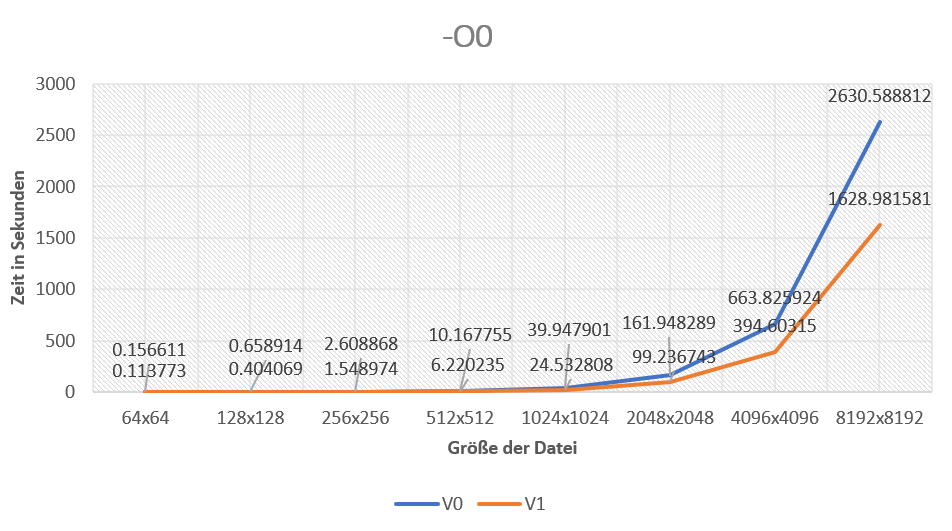
\includegraphics[scale=0.56]{images/PerformanceO0.png}
      \caption{ Performanz mit O0) \cite{Beispiel}}
    \end{center}
\end{figure}

\clearpage

\begin{figure}[!h]
    \begin{center}
      \centering
      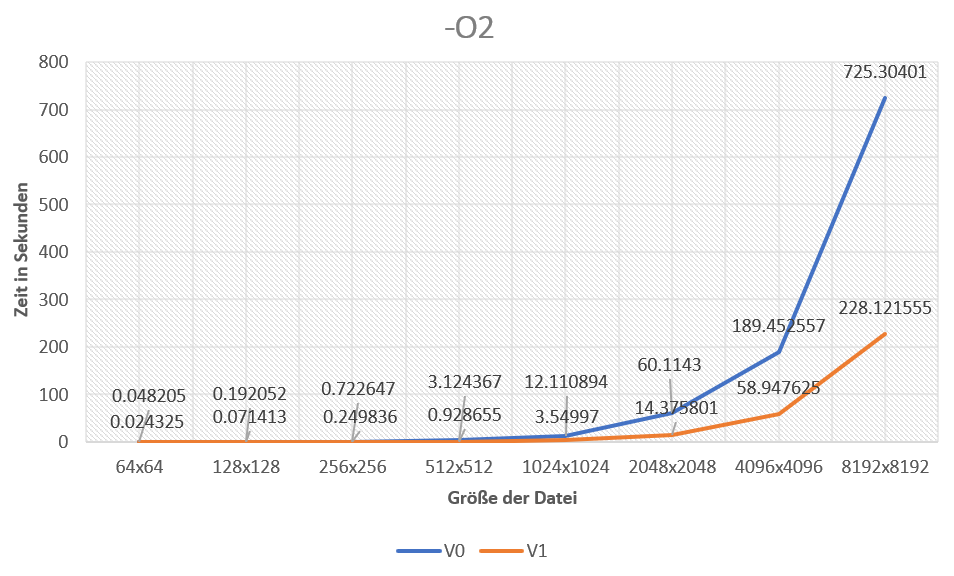
\includegraphics[scale=0.56]{images/PerformanceO1.png}
      \caption{ Performanz mit O2) \cite{Beispiel}}
    \end{center}
\end{figure}



\section{Zusammenfassung und Ausblick}

% TODO: Fuegen Sie Ihre Quellen der Datei Ausarbeitung.bib hinzu
% Referenzieren Sie diese dann mit \cite{}.
% Beispiel: CR2 ist ein Register der x86-Architektur~\cite{intel2017man}.
\bibliographystyle{plain}
\bibliography{Ausarbeitung}{}

\end{document}
